\documentclass[]{article}
\usepackage{lmodern}
\usepackage{amssymb,amsmath}
\usepackage{ifxetex,ifluatex}
\usepackage{fixltx2e} % provides \textsubscript
\ifnum 0\ifxetex 1\fi\ifluatex 1\fi=0 % if pdftex
  \usepackage[T1]{fontenc}
  \usepackage[utf8]{inputenc}
\else % if luatex or xelatex
  \ifxetex
    \usepackage{mathspec}
  \else
    \usepackage{fontspec}
  \fi
  \defaultfontfeatures{Ligatures=TeX,Scale=MatchLowercase}
\fi
% use upquote if available, for straight quotes in verbatim environments
\IfFileExists{upquote.sty}{\usepackage{upquote}}{}
% use microtype if available
\IfFileExists{microtype.sty}{%
\usepackage{microtype}
\UseMicrotypeSet[protrusion]{basicmath} % disable protrusion for tt fonts
}{}
\usepackage[margin=1in]{geometry}
\usepackage{hyperref}
\hypersetup{unicode=true,
            pdftitle={Homework \#1},
            pdfborder={0 0 0},
            breaklinks=true}
\urlstyle{same}  % don't use monospace font for urls
\usepackage{color}
\usepackage{fancyvrb}
\newcommand{\VerbBar}{|}
\newcommand{\VERB}{\Verb[commandchars=\\\{\}]}
\DefineVerbatimEnvironment{Highlighting}{Verbatim}{commandchars=\\\{\}}
% Add ',fontsize=\small' for more characters per line
\usepackage{framed}
\definecolor{shadecolor}{RGB}{248,248,248}
\newenvironment{Shaded}{\begin{snugshade}}{\end{snugshade}}
\newcommand{\KeywordTok}[1]{\textcolor[rgb]{0.13,0.29,0.53}{\textbf{#1}}}
\newcommand{\DataTypeTok}[1]{\textcolor[rgb]{0.13,0.29,0.53}{#1}}
\newcommand{\DecValTok}[1]{\textcolor[rgb]{0.00,0.00,0.81}{#1}}
\newcommand{\BaseNTok}[1]{\textcolor[rgb]{0.00,0.00,0.81}{#1}}
\newcommand{\FloatTok}[1]{\textcolor[rgb]{0.00,0.00,0.81}{#1}}
\newcommand{\ConstantTok}[1]{\textcolor[rgb]{0.00,0.00,0.00}{#1}}
\newcommand{\CharTok}[1]{\textcolor[rgb]{0.31,0.60,0.02}{#1}}
\newcommand{\SpecialCharTok}[1]{\textcolor[rgb]{0.00,0.00,0.00}{#1}}
\newcommand{\StringTok}[1]{\textcolor[rgb]{0.31,0.60,0.02}{#1}}
\newcommand{\VerbatimStringTok}[1]{\textcolor[rgb]{0.31,0.60,0.02}{#1}}
\newcommand{\SpecialStringTok}[1]{\textcolor[rgb]{0.31,0.60,0.02}{#1}}
\newcommand{\ImportTok}[1]{#1}
\newcommand{\CommentTok}[1]{\textcolor[rgb]{0.56,0.35,0.01}{\textit{#1}}}
\newcommand{\DocumentationTok}[1]{\textcolor[rgb]{0.56,0.35,0.01}{\textbf{\textit{#1}}}}
\newcommand{\AnnotationTok}[1]{\textcolor[rgb]{0.56,0.35,0.01}{\textbf{\textit{#1}}}}
\newcommand{\CommentVarTok}[1]{\textcolor[rgb]{0.56,0.35,0.01}{\textbf{\textit{#1}}}}
\newcommand{\OtherTok}[1]{\textcolor[rgb]{0.56,0.35,0.01}{#1}}
\newcommand{\FunctionTok}[1]{\textcolor[rgb]{0.00,0.00,0.00}{#1}}
\newcommand{\VariableTok}[1]{\textcolor[rgb]{0.00,0.00,0.00}{#1}}
\newcommand{\ControlFlowTok}[1]{\textcolor[rgb]{0.13,0.29,0.53}{\textbf{#1}}}
\newcommand{\OperatorTok}[1]{\textcolor[rgb]{0.81,0.36,0.00}{\textbf{#1}}}
\newcommand{\BuiltInTok}[1]{#1}
\newcommand{\ExtensionTok}[1]{#1}
\newcommand{\PreprocessorTok}[1]{\textcolor[rgb]{0.56,0.35,0.01}{\textit{#1}}}
\newcommand{\AttributeTok}[1]{\textcolor[rgb]{0.77,0.63,0.00}{#1}}
\newcommand{\RegionMarkerTok}[1]{#1}
\newcommand{\InformationTok}[1]{\textcolor[rgb]{0.56,0.35,0.01}{\textbf{\textit{#1}}}}
\newcommand{\WarningTok}[1]{\textcolor[rgb]{0.56,0.35,0.01}{\textbf{\textit{#1}}}}
\newcommand{\AlertTok}[1]{\textcolor[rgb]{0.94,0.16,0.16}{#1}}
\newcommand{\ErrorTok}[1]{\textcolor[rgb]{0.64,0.00,0.00}{\textbf{#1}}}
\newcommand{\NormalTok}[1]{#1}
\usepackage{longtable,booktabs}
\usepackage{graphicx,grffile}
\makeatletter
\def\maxwidth{\ifdim\Gin@nat@width>\linewidth\linewidth\else\Gin@nat@width\fi}
\def\maxheight{\ifdim\Gin@nat@height>\textheight\textheight\else\Gin@nat@height\fi}
\makeatother
% Scale images if necessary, so that they will not overflow the page
% margins by default, and it is still possible to overwrite the defaults
% using explicit options in \includegraphics[width, height, ...]{}
\setkeys{Gin}{width=\maxwidth,height=\maxheight,keepaspectratio}
\IfFileExists{parskip.sty}{%
\usepackage{parskip}
}{% else
\setlength{\parindent}{0pt}
\setlength{\parskip}{6pt plus 2pt minus 1pt}
}
\setlength{\emergencystretch}{3em}  % prevent overfull lines
\providecommand{\tightlist}{%
  \setlength{\itemsep}{0pt}\setlength{\parskip}{0pt}}
\setcounter{secnumdepth}{0}
% Redefines (sub)paragraphs to behave more like sections
\ifx\paragraph\undefined\else
\let\oldparagraph\paragraph
\renewcommand{\paragraph}[1]{\oldparagraph{#1}\mbox{}}
\fi
\ifx\subparagraph\undefined\else
\let\oldsubparagraph\subparagraph
\renewcommand{\subparagraph}[1]{\oldsubparagraph{#1}\mbox{}}
\fi

%%% Use protect on footnotes to avoid problems with footnotes in titles
\let\rmarkdownfootnote\footnote%
\def\footnote{\protect\rmarkdownfootnote}

%%% Change title format to be more compact
\usepackage{titling}

% Create subtitle command for use in maketitle
\newcommand{\subtitle}[1]{
  \posttitle{
    \begin{center}\large#1\end{center}
    }
}

\setlength{\droptitle}{-2em}
  \title{Homework \#1}
  \pretitle{\vspace{\droptitle}\centering\huge}
  \posttitle{\par}
  \author{Stat4DS2+DS\\
\url{https://elearning2.uniroma1.it/course/view.php?id=4951}}
  \preauthor{\centering\large\emph}
  \postauthor{\par}
  \predate{\centering\large\emph}
  \postdate{\par}
  \date{\textbf{deadline 23/03/2017 (23:55)}}

\usepackage{graphicx}

\begin{document}
\maketitle

{
\setcounter{tocdepth}{2}
\tableofcontents
}
\begin{longtable}[]{@{}l@{}}
\toprule
Your Last+First Name \_\_MELE\_\emph{UMBERTO\_Jr} Your Matricola
\emph{1388371}\tabularnewline
\midrule
\endhead
\newpage\tabularnewline
\bottomrule
\end{longtable}

1a) Illustrate the characteristics of the statistical model for dealing
with the \emph{Dugong}'s data. Ages (\(Y_i\)) and lengths (\(x_i\)) of
27 Dugongs have been recorded and the following (non linear) regression
model is considered:

\begin{eqnarray*}
Y_i &\sim& N(\mu_i, \tau^2) \\
\mu_i=f(x_i)&=& \alpha - \beta \gamma^{x_i}\\
\end{eqnarray*}

Model parameters are \(\alpha \in (1, \infty)\),
\(\beta \in (1, \infty)\), \(\gamma \in (0,1)\),
\(\tau^2 \in (0,\infty)\). Let us consider the following prior
distributions:

\begin{eqnarray*}
\alpha &\sim&  N(0,\sigma^2_{\alpha})\\
\beta  &\sim&  N(0,\sigma^2_{\beta}) \\
\gamma &\sim&  Unif(0,1)\\
\tau^2 &\sim&  IG(a,b)) (Inverse Gamma)
\end{eqnarray*}

\begin{verbatim}
## 
## Attaching package: 'igraph'
\end{verbatim}

\begin{verbatim}
## The following objects are masked from 'package:stats':
## 
##     decompose, spectrum
\end{verbatim}

\begin{verbatim}
## The following object is masked from 'package:base':
## 
##     union
\end{verbatim}

\includegraphics[width=500px]{1388371_mele_files/figure-latex/unnamed-chunk-1-1}

1b) Derive the corresponding likelihood function

1c) Write down the expression of the joint prior distribution of the
parameters at stake and illustrate some suitable choice for the
hyperparameters.

1d) Compute \underline{numerically} the maximum likelihood estimate for
the vector of parameters of interest
\((\alpha , \beta , \gamma , \tau)\) and compare it with the
Maximum-a-Posterori estimate

(\emph{write your answers and provide your R code for the numerical
solution})

\begin{Shaded}
\begin{Highlighting}[]
\CommentTok{#}
\CommentTok{#}
\CommentTok{#}
\CommentTok{#}
\CommentTok{#}
\CommentTok{#}
\CommentTok{#}
\CommentTok{#}
\CommentTok{#}
\end{Highlighting}
\end{Shaded}

\newpage

\begin{enumerate}
\def\labelenumi{\arabic{enumi})}
\setcounter{enumi}{1}
\tightlist
\item
  Consider the Acceptance-Rejection algorithm in the most general form
  and denote with \(\theta=Y^A\) the random variable obtained with the
  algorithm
\end{enumerate}

2a) Determine the analytic expression of the acceptance probability

2b) Prove that \(\theta\) has the desired target distribution

2c) Show how in Bayesian inference you could use simulations from the
prior (auxiliary density) to get a random draw from the posterior
(target distribution) without knowing the proportionality constant

2d) Illustrate analytically possible difficulties of this approach with
a simple conjugate model

2e) Verify your conclusions implementing the Acceptance-Rejection
approach with your conjugate model (verify empirically that \(\theta\)
has the desired target distribution \(\pi(\theta|x_1,..,x_n)\)

(\emph{write your answer; provide your R code for the last point})

\begin{Shaded}
\begin{Highlighting}[]
\CommentTok{#}
\CommentTok{#}
\CommentTok{#}
\CommentTok{#}
\CommentTok{#}
\CommentTok{#}
\CommentTok{#}
\CommentTok{#}
\CommentTok{#}
\end{Highlighting}
\end{Shaded}

\newpage

\begin{enumerate}
\def\labelenumi{\arabic{enumi})}
\setcounter{enumi}{2}
\tightlist
\item
  Simulate from a standard Normal distribution using pseudo-random
  deviates from a standard Cauchy and the A-R algorithm. Write the
  expression the corresponding acceptance probabilityof and evaluate it
  numerically by MC approximation.
\end{enumerate}

\begin{Shaded}
\begin{Highlighting}[]
\CommentTok{#}
\CommentTok{#}
\CommentTok{#}
\CommentTok{#}
\CommentTok{#}
\CommentTok{#}
\CommentTok{#}
\CommentTok{#}
\CommentTok{#}
\end{Highlighting}
\end{Shaded}

\newpage

\begin{enumerate}
\def\labelenumi{\arabic{enumi})}
\setcounter{enumi}{3}
\tightlist
\item
  Let us consider a Markov chain \((X_t)_{t \geq 0}\) defined on the
  state space \({\cal S}=\{1,2,3\}\) with the following transition
\end{enumerate}

\begin{center} 
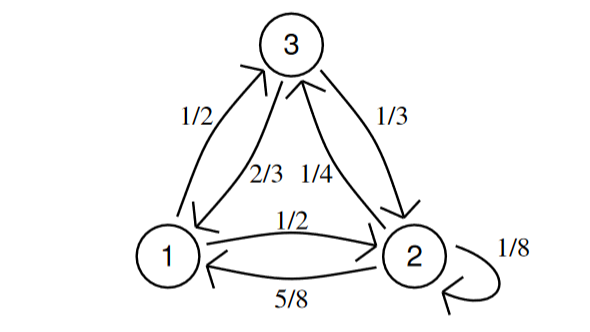
\includegraphics[width=6cm]{frog.png} 
\end{center}

4a) Starting at time \(t=0\) in the state \(X_0=1\) simulate the Markov
chain with distribution assigned as above for \(t=1000\) consecutive
times

4b) compute the empirical relative frequency of the two states in your
simulation 4c) repeat the simulation for 500 times and record only the
final state at time \(t=1000\) for each of the 500 simulated chains.
Compute the relative frequency of the 500 final states. What
distribution are you approximating in this way?\\
Try to formalize the difference between this point and the previous
point.

4d) compute the theoretical stationary distribution \(\pi\) and explain
how you have obtained it

4e) is it well approximated by the simulated empirical relative
frequencies computed in (b) and (c)?

4f) what happens if we start at \(t=0\) from state \(X_0=2\) instead of
\(X_0=1\)?

\begin{Shaded}
\begin{Highlighting}[]
\CommentTok{#}
\CommentTok{#}
\CommentTok{#}
\CommentTok{#}
\CommentTok{#}
\CommentTok{#}
\CommentTok{#}
\CommentTok{#}
\CommentTok{#}
\end{Highlighting}
\end{Shaded}

\newpage

\begin{enumerate}
\def\labelenumi{\arabic{enumi})}
\setcounter{enumi}{4}
\tightlist
\item
  Consider again the Bayesian model for Dugong's data:
\end{enumerate}

5a) Derive the functional form (up to proportionality constants) of all
\emph{full-conditionals}

5b) Which distribution can you recognize within standard parametric
families so that direct simulation from full conditional can be easily
implemented ?

5c) Using a suitable Metropolis-within-Gibbs algorithm simulate a Markov
chain (\(T=10000\)) to approximate the posterior distribution for the
above model

5d) Show the 4 univariate trace-plots of the simulations of each
parameter

5e) Evaluate graphically the behaviour of the empirical averages
\(\hat{I}_t\) with growing \(t=1,...,T\)

5f) Provide estimates for each parameter together with the approximation
error and explain how you have evaluated such error

5g) Which parameter has the largest posterior uncertainty? How did you
measure it?

5h) Which couple of parameters has the largest correlation (in absolute
value)?

5i) Use the Markov chain to approximate the posterior predictive
distribution of the length of a dugong with age of 20 years.

5j) Provide the prediction of another dugong with age 30

5k) Which prediction is less precise?

\begin{Shaded}
\begin{Highlighting}[]
\CommentTok{#}
\CommentTok{#}
\CommentTok{#}
\CommentTok{#}
\CommentTok{#}
\CommentTok{#}
\CommentTok{#}
\CommentTok{#}
\CommentTok{#}
\end{Highlighting}
\end{Shaded}

\vspace*{6cm}

\begin{center}\rule{0.5\linewidth}{\linethickness}\end{center}

© 2016-2017 - Stat4DS2+CS - Luca Tardella

\begin{verbatim}
## This homework will be graded and it will be part of your final evaluation 
## 
## 
\end{verbatim}

\begin{verbatim}
## Last update by LT: Sun May 07 20:33:48 2017
\end{verbatim}


\end{document}
